\documentclass[tikz,border=3mm]{standalone}
\usetikzlibrary{chains, calc,fit}
\usepackage{varwidth}
\begin{document}
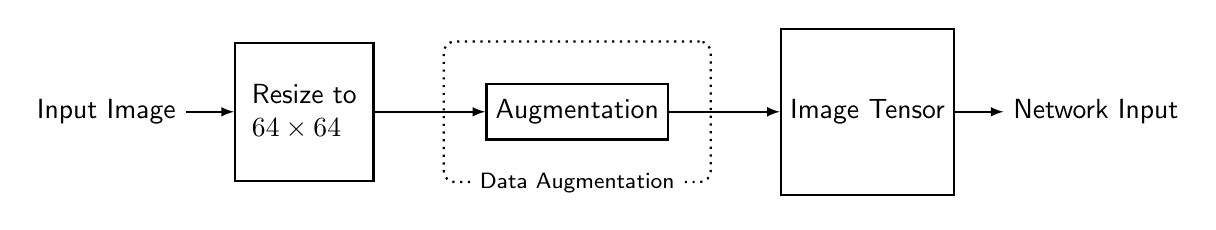
\begin{tikzpicture}[box/.style={draw,thick,minimum width=5em,minimum
    height=10em},arj/.style={semithick,-latex}]
  \begin{scope}[start chain=A going right,oc/.style={join=by arj,on chain},
    font=\sffamily,node distance=1.75em]
   \node(data)[oc]{Input Image};
   \node(data resizing)[box,minimum height=5em,oc]{
   \begin{varwidth}{5em}
    Resize to \\ $64\times 64$
   \end{varwidth}
   };
   \node(augment)[box, minimum height = 2em, minimum width=2em,oc][right=4em of data resizing]{Augmentation};
   \node(conversion)[box,minimum height=6em,minimum width=6em,oc][right=4em of augment]{Image Tensor};
   \node(output)[oc]{Network Input};
   \node[draw, thick, dotted, rounded corners, inner xsep=1.5em, inner ysep=1.5em, fit=(augment)] (box) {};
   \node[fill=white] at (box.south) {\footnotesize Data Augmentation};
  \end{scope}
  
%   \begin{scope}[shift = {{($(input.south)+(0cm, -2cm)$)}}, start chain=A going right, oc/.style={join=by arj, on chain},
%     font=\sffamily, node distance=1.75em]
%     \node[box,oc]{something};
%   \end{scope}
\end{tikzpicture}
\end{document}